\documentclass{tufte-handout}
\usepackage{amsmath}
\pagestyle{empty}
\usepackage[utf8]{inputenc}
\usepackage{mathpazo}
\usepackage{booktabs}
\usepackage{microtype}
\usepackage{xcolor}

\usepackage{tikz}
\usetikzlibrary{matrix}
\usetikzlibrary{chains}
\usetikzlibrary{decorations}

\input{vc.tex}

\title{Runsort}
\author{Thore Husfeldt}
\date{\small Revision \GITAbrHash, \GITAuthorDate}


\begin{document}

\maketitle
\subsection{Sorting by runs}

This exercise asks you to implement a sorting algorithm that we call \emph{runsort}.
The main goal of the exercise is to expose you to the details of correctly implementing a nontrivial sorting algorithm.
This includes careful index manipulation, special cases, and memory management.
The algorithm shares many features with \emph{bottom-up mergesort}, and you are welcome to re-use as much of the code in our textbook\sidenote{R. Sedgewick and K. Wayne, \emph{Algorithms}, 4th ed., Addison--Wesley, 2011.} as you deem useful, in particular from section 2.2.

\medskip
A \emph{run} in a subsequence is a maximal sequence of nondecreasing, consecutive elements.
For instance, the runs in  \texttt{RUNSORTEXAMPLE} are \texttt{RU}, \texttt{NS}, \texttt{ORT}, \texttt{EX}, \texttt{AMP}, \texttt{L}, and \texttt{E}.
There are two runs in \texttt{ZOO}, namely \texttt{Z} and \texttt{OO}.
A sequence is sorted if and only if it consists of a single run.

Runsort works in rounds.
Each round merges pairs of neighbouring runs.
(If the number of runs is odd, the last run is not merged.)
Each round divides the number of runs by 2, so after $\sim\!\operatorname{lg} N$ rounds, the process stops.
See Fig.~\ref{fig: runsort}.


\begin{figure*}
\newcommand{\hhlline}[3]{\draw (#1-#2-1.south west) -- (#1-#2-#3.south east);}
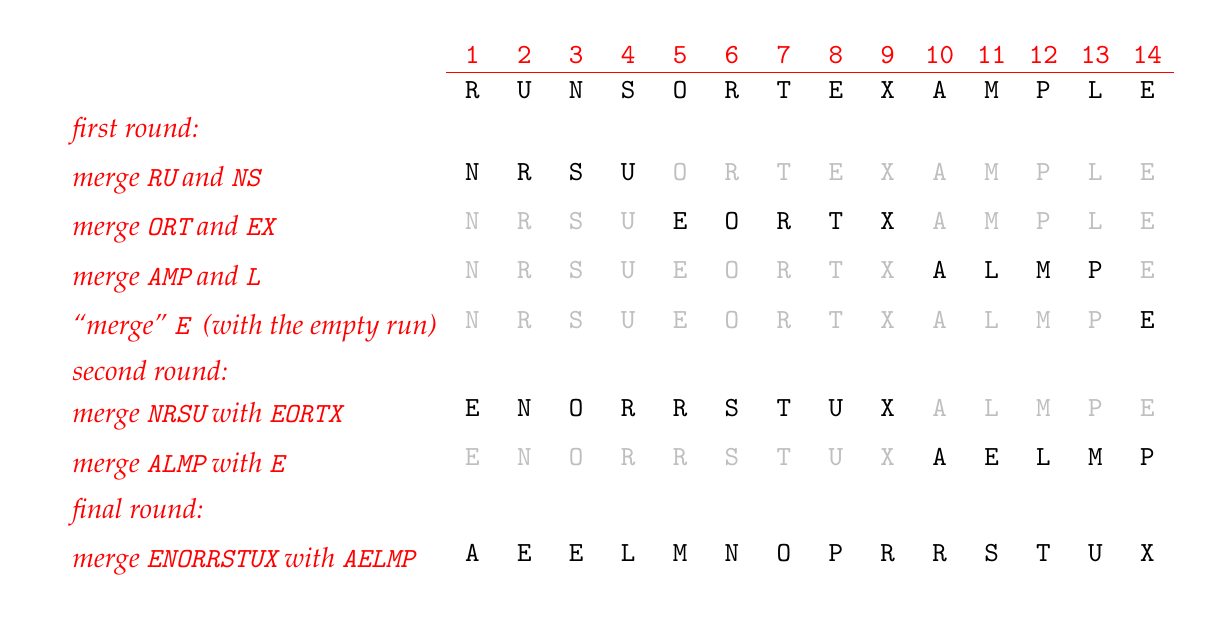
\begin{tikzpicture}[scale=.9]
  \tikzstyle{b}=[black] % black entries have just been changed
  \tikzstyle{com}=[right,red, font={\rmfamily\itshape}] % comments are in red italics
  \node[
    matrix of nodes,
    nodes in empty cells,
    nodes ={font=\ttfamily, minimum width =4ex},
    row 1/.style={red},
    row 4/.style={black!25},
    row 5/.style={black!25},
    row 6/.style={black!25},
    row 7/.style={black!25},
    row 9/.style={black!25},
    row 10/.style={black!25}
    ]
    (t) {
                                   &  1 & 2 & 3 & 4 & 5 & 6 & 7 & 8 & 9 & 10 & 11 & 12 & 13 & 14 \\
                                   &  R & U & N & S & O & R & T & E & X & A & M & P & L & E \\
    |[com]|first round:\\
    |[com]|merge \texttt{RU} and \texttt{NS}
                                  &  |[b]| N & |[b]| R & |[b]| S & |[b]| U &  O& R&T&E&X&A&M&P&L&E\\
    |[com]|merge \texttt{ORT} and \texttt{EX} &   N &  R & S & U &  |[b]|E&|[b]|O& |[b]|R&|[b]|T&|[b]|X   &A&M&P&L&E\\
    |[com]|merge \texttt{AMP} and \texttt{L} &   N &  R & S & U &  E&O& R&T&X   &|[b]|A&|[b]|L&|[b]|M&|[b]|P&E\\
    |[com]|``merge'' \texttt{E} \/ (with the empty run) &   N &  R & S & U &  E&O& R&T&X   &A&L&M&P&|[b]|E\\
    |[com]|second round:\\
    |[com]|merge \texttt{NRSU} with \texttt{EORTX}  &   |[b]|E & |[b]|N &  |[b]|O&|[b]|R &|[b]|R&|[b]| S & |[b]|T& |[b]|U &|[b]|X   &A&L&M&P&E\\
    |[com]|merge \texttt{ALMP} with \texttt{E}  &   E & N &  O&R &R& S & T& U &X   &|[b]|A&|[b]|E&|[b]|L&|[b]|M&|[b]|P\\
    |[com]|final round:\\
    |[com]|merge \texttt{ENORRSTUX} with \texttt{AELMP}  &   A&E&E&L&M&N&O&P&R&R&S&T&U&X\\
};
\draw [red] (t-1-2.south west) -- (t-1-15.south east);
\end{tikzpicture}
\caption{\label{fig: runsort}Trace of runsort}
\end{figure*}


\subsection{Requirements}
Write an implementation of runsort in Java.
Follow the conventions used in the textbook:
\begin{enumerate}
\item Write a class \texttt{Runsort} that includes a method
\texttt{public static void sort(Comparable[] a)}.
\item You must use the method \texttt{less} from the \texttt{Example} class in section 2.1 and  simple array manipulation.
\footnote{Since runsort isn't an in-place sorting algorithm, we  need an auxiliary array.
In particular, the \texttt{exch} method from the \texttt{Example} class won't be enough for our purposes.
Just like for mergesort.}
\item You are not allowed to use more than linear extra space.
\end{enumerate}

\subsection{Tips and comments}
\begin{enumerate}
\item As always, do not reinvent the wheel, for your own sake as much as ours.
For instance, I used the \texttt{merge} method from section 2.2 in the textbook without modification, including the neat trick with a static \texttt{aux} array for auxiliary storage.
When reusing code, remember to be open about it (for instance, add a comment like ``from Sedgewick and Wayne, section 2.2.'' to your code).\sidenote{Indeed, one of the goals of this exercise is to motivate you to understand what's happening in the book's mergesort code.}
\item I solved this exercise using 30 lines of my own code, and maybe 30 lines from \texttt{MergeBU}.
Most of the time I spent on hunting annoying index mistakes.
\item Test your code using the client in \texttt{Example} in section 2.1.
Make sure you've run your sorting algorithm on \texttt{tiny.txt} and \texttt{words3.txt}, but also on some pathological cases: empty input, 1-letter input, 2-letter input, etc.
Also, sort something really big.
\end{enumerate}


\subsection{Bells and whistles}
Implement at least one of the following fancy extensions.
\begin{enumerate}
\item \emph{Insertions sort to avoid short runs.}
  Never merge runs that are shorter than 8 elements.
  If the current run length is less than 8,
  use insertion sort to sort the next 8 positions.\sidenote{There's nothing magical about 8.
  In fact, larger values like 32 or 64 are probably better.
  But then the whole algorithm becomes hard to debug, because most of your test inputs will be too short to ever use the merge step.}
\item \emph{Mirror down-runs.}
  When scanning for runs, also check \emph{decreasing} runs (such as \texttt{ZMFCBA}).
  Whenever you find a decreasing run, revert it in linear time.
  This trick makes the algorithm run much bfaster on almost-reverse-sorted input.
\item \emph{Galloping.} Read Peters\sidenote{Tim Peters, \emph{timsort.txt}, bugs.python.org/file4451/timsort.txt. Retrieved 11 March 2014.} or Wikipedia\sidenote{Timsort, \emph{Wikipedia, The Free Encyclopedia}. Wikimedia Foundation, Inc. Retrieved 11 March 2014.}. Good luck!
\item Draw a visual trace of runsort for each round in the style of the book, e.g., like the ``Visual trace of shellsort'' figure in section 2.1.
  (\texttt{StdStats.plotBars} does most the work for you.)
\end{enumerate}

\subsection{Deliverables}

\begin{enumerate}
  \item The java source code for Runsort.
      Make sure it's perfect, following the book's conventions for clarity, brevity, indentation, variable names, comments, etc.
  \item A report in PDF.
  Use the report skeleton on the next page.
  \item Any input files that gave your sorting algorithm trouble.
\end{enumerate}

\subsection{Further reading}
Runsort sometimes called of polyphase merge sort\sidenote{Polyphase merge sort, \emph{Wikipedia, The Free Encyclopedia}. Wikimedia Foundation, Inc. Retrieved 11 March 2014.} or natural merge sort\sidenote{Sedgewick and Wayne, exercise 2.2.16}.
With most of the ideas mentioned above, and a few more due to Tim Peters, it is used in Python (since version 2.3) and Java (since SE 7), often called Timsort.

\newpage
\section{Runsort Report}


by Alice Cooper and Bob Marley\sidenote{Complete the report by filling
  in your names and the parts marked $[\ldots]$.
  Remove the sidenotes in your final hand-in.}

  \subsection{Tests}
  We have run our sorting algorithm on the following inputs from the book; all were sorted:
    {\tt tiny.txt}, {\tt words3.txt},  $[\ldots]$

  We also ran our sorting algorithm on {\tt cannotsort.txt} (included).
  The algorithm fails on this input, but we cannot find the error in our code.\sidenote{Edit or remove this paragraph if you were unable to find an input where your sorting algorithm failed.}

  \subsection{Extensions}  \sidenote{In this section, briefly state which extension you chose to implement, and (if it makes sense) report on a single, simple experiment.}

  Our implementation switches to insertion sort for sequences of length at most 8.
  We performed test with and without this extension for random inputs of size 1,000,000, but
  we were not able to detect any improvement in running time.
  \sidenote{Remove or edit as necessary.
  Perform the empirical test and report the result.
  If you want, try with various sequence lengths and various input lengths.
  Maybe report the running times in the form of a graph or table.
  Or write ``Unfortunately, with this extension, our code no longer sorts correctly and we are unable to find the error.''
  }

  Our implementation mirrors down-runs.
    This gives a significant improvement on inputs that $[\ldots]$.
  For instance, the improved code sorts an input consisting of $[\ldots]$ in time
  $[\ldots]$, whereas the original implementation used $[\ldots]$. \sidenote{Remove or edit as necessary.}

  We attempted to understand \emph{galloping}, and have implemented the following idea: $[\ldots]$.
  The result was great on {\tt somefile.txt} (included), but we weren't able to detect any improvement on other inputs. \sidenote{Remove or edit as necessary.}


  The figure below shows a visual trace of runsort:
  $[\ldots]$.

\end{document}
